This section focuses on the design of the map representation used in the multi-agent system. The map serves as a representation of the possible location of the agents in a discrete space. The initial map generated for the agents will indicate the starting and finishing points for each agent. Additionally, different algorithms may require the map to be translated into different forms, such as a graph. These different forms of representation are necessary to enable the efficient operation of specific algorithms. 

\subsection{Gridmap}
A grid map represents the potential locations of an agent in a discrete space. The starting and ending points for each agent are marked on the initial map, along with areas that are inaccessible, referred to as "walls" or "obstacles". Two map formats will be implemented: a space-separated map for creating and storing persistent maps and a human-readable format, and a JSON-based map for machine-to-machine communication and ease of parsing. The map service will handle the conversion and storage of maps, and will serve them to the agents, including the ability to generate random maps and place agents on them.

\begin{figure}[H]
    \centering
    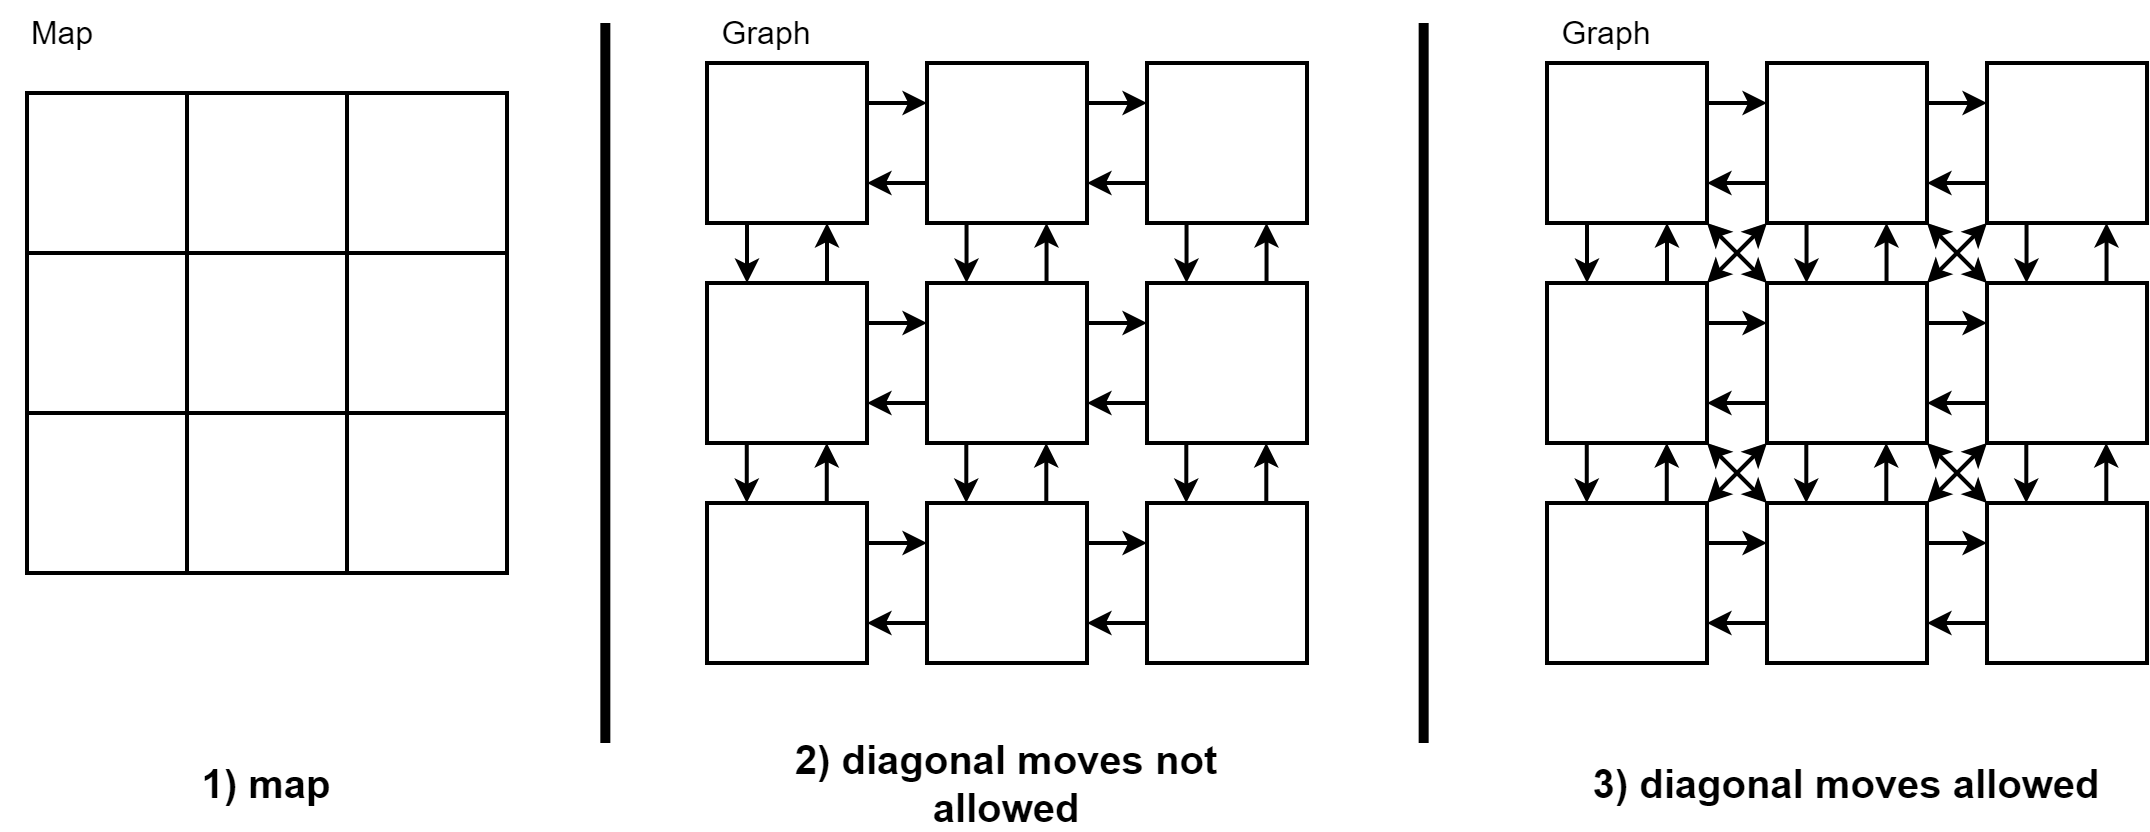
\includegraphics[width=\textwidth]{pictures/map_2d.png}
    \caption{2D map to graph translation}
    \label{fig:map_2D}
\end{figure}

Each tile represents the node and it is connected with two edges to neighboring tiles, which represents the possibility of two-way movement from and to neighboring tiles. 


\subsection{Gridmap for CA* algorithm}
For CA* algorithm map has to be translated into a three dimensional(3D) grid map where every layer is a representation of the possible location of the agent in a particular time frame and therefore time becomes the third dimension in a graph. Similar to in a 2d grid map there are two possible modes which are represented in the figure below. An agent can only move in one direction vertically as each level corresponds to one moment in time. Other tiles on each level are connected in the same way as in figure \ref{fig:map_2D}.
\begin{figure}[H]
    \centering
    \includegraphics[width=\textwidth]{pictures/map_3D.png}
    \caption{3D map to graph translation}
    \label{fig:map_3D}
\end{figure}
After the path is planned for specific agents, it has to be marked as an obstacle so agents which are planning their paths, later on, would be aware of unreachable/occupied tiles.

\subsection{CA* front collision problem}
Planning multiple agents' paths on a single map leads to a problem when agents are colliding with each other because they are moving in the opposite direction on the same column or row. This situation is shown in Figure \ref{fig:head_collision}. Both agents assume that the tile in front of them is not occupied, which is a valid assumption. However, as this is a discrete model, a collision occurs between timeframes. To mitigate this problem, after the path is planned edges in the opposite direction of agent movement need to be removed.
\begin{figure}[H]
    \centering
    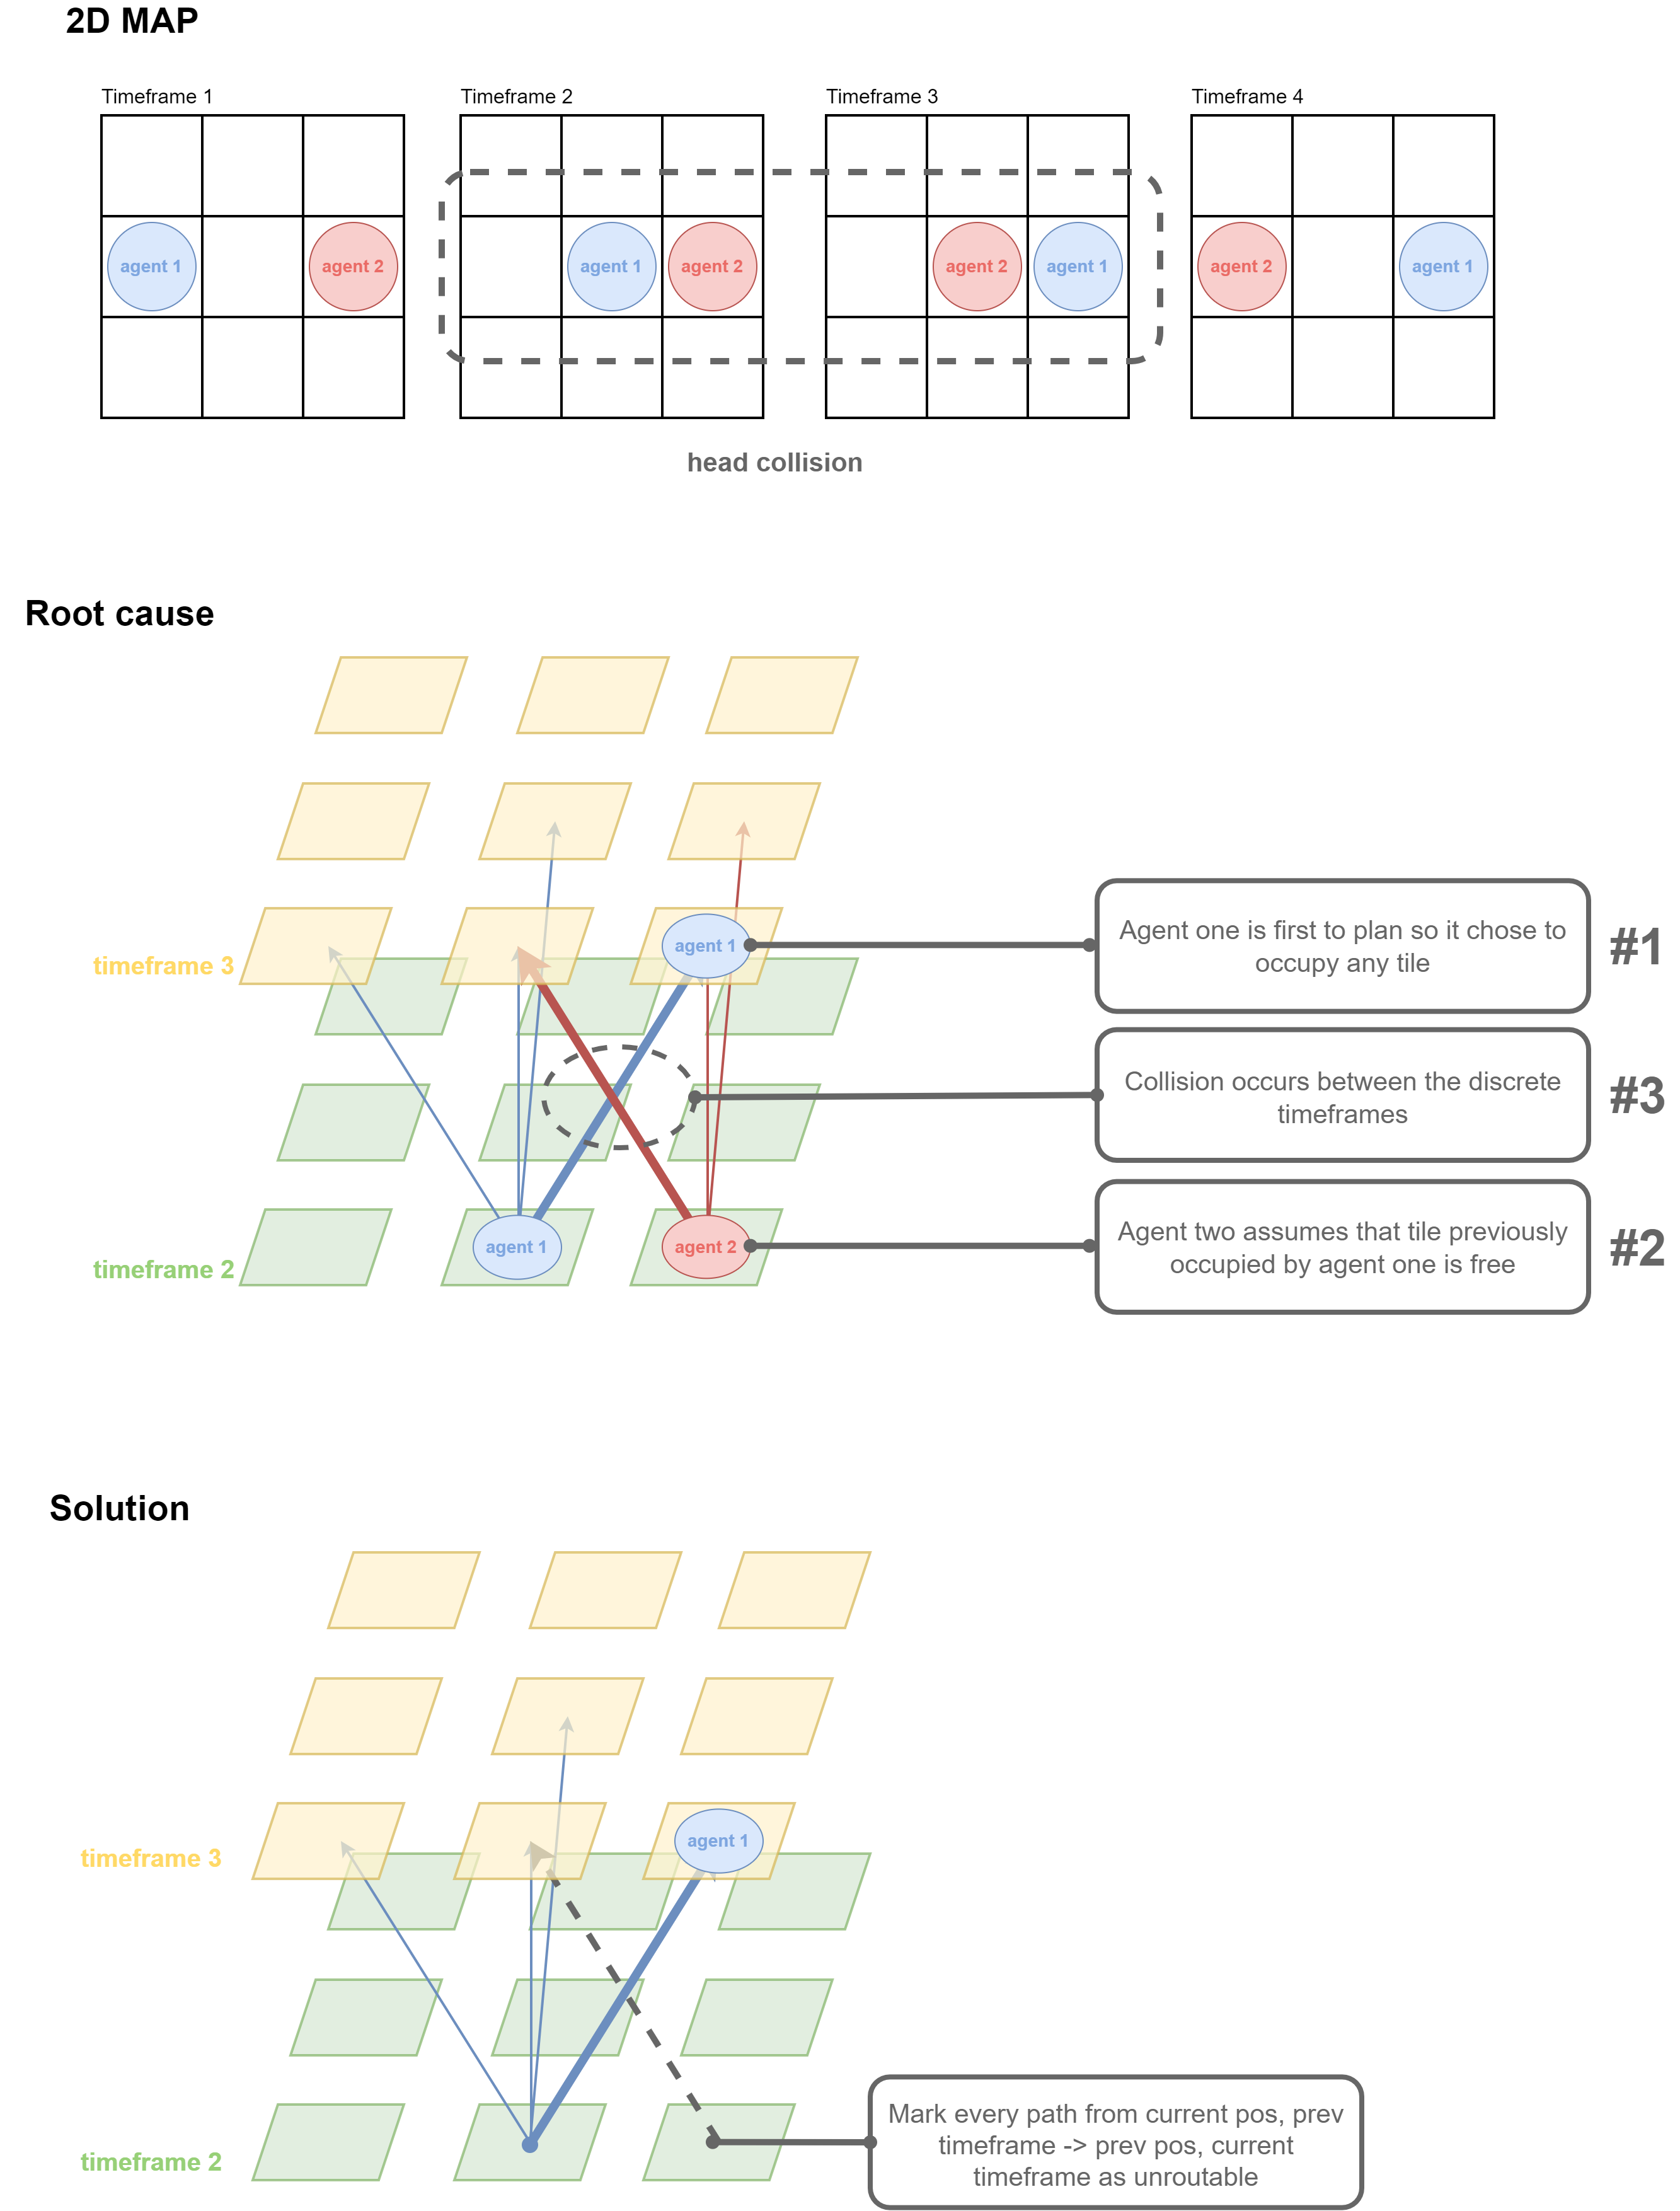
\includegraphics[width=0.7\textwidth]{pictures/head_collision_problem.png}
    \caption{CA* head collision problem}
    \label{fig:head_collision}
\end{figure}